% ============================================================
%  Ask What Matters — Pitch Deck
%  2026 Wharton Hack-AI-thon | Expedia Group
% ============================================================
\documentclass[aspectratio=169,10pt]{beamer}

\usepackage[T1]{fontenc}
\usepackage[utf8]{inputenc}
\usepackage{lmodern}
\usepackage{microtype}
\usepackage{amsmath}
\usepackage{tikz}
\usetikzlibrary{arrows.meta}

% ── Theme ────────────────────────────────────────────────────
\usetheme{default}

\setbeamerfont{frametitle}{size=\large, series=\bfseries}

\setbeamertemplate{navigation symbols}{}
\setbeamertemplate{footline}{%
  \begin{beamercolorbox}[wd=\paperwidth,ht=2ex,dp=1ex]{normal text}%
    \hspace{1em}\tiny Team 375\hfill\tiny\insertframenumber\hspace{1em}
  \end{beamercolorbox}%
}
\setbeamertemplate{frametitle}{%
  \vspace{0.4em}%
  \hyphenpenalty=10000\exhyphenpenalty=10000%
  \insertframetitle\par%
  \vspace{-0.2em}%
  \rule{\textwidth}{0.4pt}\par%
  \vspace{0.15em}%
}

% ── TikZ styles ──────────────────────────────────────────────
\tikzset{
  arr/.style={->, >=Stealth, semithick},
  wbox/.style={draw, rounded corners=2pt, text centered, font=\scriptsize,
               inner sep=5pt, text width=1.9cm, minimum height=0.65cm},
  lbox/.style={draw, rounded corners=2pt, text centered, font=\scriptsize,
               inner sep=3pt, text width=1.7cm, minimum height=0.58cm},
}

% ── Helpers ──────────────────────────────────────────────────
\newcommand{\shead}[1]{\smallskip\textbf{#1}\par\smallskip}
\newcommand{\arrow}{$\rightarrow$}

% ── Title info ───────────────────────────────────────────────
\title{\textbf{Ask What Matters}}
\subtitle{Closing the Information Gap in Hotel Reviews}
\author{2026 Wharton Hack-AI-thon \textbar{} Expedia Group \textbar{} Team 375}
\date{}

% ============================================================
\begin{document}
% ============================================================

% ── Slide 1: Title ───────────────────────────────────────────
\begin{frame}
\titlepage
\end{frame}

% ── Slide 2: Problem ─────────────────────────────────────────
\begin{frame}{Reviews Are the Most Trusted Signal --- and the Most Incomplete One}

\textit{``I want a hotel with a quiet room and good blackout curtains --- but nobody writes about that.''}

\medskip
81\% of travelers say reviews are important when choosing accommodation (TripAdvisor/Ipsos, 2023).
Yet review content is almost entirely \textbf{supply-driven}:
reviewers write what they remember, not what future guests need to know.

\medskip
\shead{Two failure modes}
\begin{itemize}
  \item \textbf{Sparseness} --- critical topics (noise, accessibility, check-in) go unmentioned
  \item \textbf{Conflict} --- reviews contradict each other on the same topic, leaving prospective guests unable to form a reliable picture
\end{itemize}

\medskip
Both reduce booking confidence, drive pre-stay support contacts, and depress conversion on
properties whose quality the review corpus simply fails to convey.

\end{frame}

% ── Slide 3: Two approaches fail ─────────────────────────────
\begin{frame}{Two Obvious Approaches --- and Why Both Fall Short}

\begin{columns}[T]
\column{0.48\textwidth}
\shead{Structured inline prompts (current standard)}
Topic tags, subcategory ratings, guided fields in the review form.
\begin{itemize}
  \item Captures platform-defined categories --- not what \textit{this} traveler needs to know
  \item Static and universal: don't adapt to what people are asking about this property now
  \item Optimises for data collection, not traveler-to-traveler information transfer
\end{itemize}

\column{0.48\textwidth}
\shead{Voice collection}
We deliberately chose not to implement voice.
\begin{itemize}
  \item Reviewers write \textbf{because they enjoy writing} --- tone, word choice, punctuation are part of the experience
  \item Voice turns a writer into a respondent; the review becomes a transcript
  \item Altruism and enjoyment of writing are primary review motives (Yoo \& Gretzel 2008); obligatory or intrusive prompts risk crowding out that intrinsic motivation (Evans et al.\ 2019)
\end{itemize}
\end{columns}

\smallskip
\textbf{Neither approach routes what travelers need to know back to the people who can answer it.}

\end{frame}

% ── Slide 4: The insight ─────────────────────────────────────
\begin{frame}{The Insight: Altruism Already Exists --- It Just Needs Direction}

Review-writing is primarily motivated by \textbf{altruism} --- the desire to help fellow travelers
(Llorens-Mar\'in 2023; Yoo \& Gretzel 2008; Hennig-Thurau et al.\ 2004).
Reviewers don't need to be pushed harder. They need to be \textit{shown what's missing}.

\medskip
\shead{Design constraints that follow}
\begin{itemize}
  \item \textbf{Non-coercive framing:} ``here is what others still want to know'' activates prosocial intent;
        ``please complete these fields'' triggers resistance (Evans et al.\ 2019)
  \item \textbf{Start of flow:} the nudge must appear before composition begins, when altruistic intent
        is highest --- post-submission follow-ups arrive after motivation is discharged
  \item \textbf{Text stays text:} habit and ease-of-use are strong drivers of repeat review contribution;
        adding friction or changing the medium risks suppressing both (Dogra 2019; Bakshi 2021)
  \item \textbf{Visible, ignorable, never blocking:} the cost of ignoring the nudge must be zero
\end{itemize}

\medskip
\textbf{Every design decision in Ask What Matters follows directly from these constraints.}

\end{frame}

% ── Slide 5: Solution ────────────────────────────────────────
\begin{frame}{Ask What Matters: A Two-Sided Information System}

\shead{Feature 1 --- Reviewer Gap Panel (Supply Side)}
When a reviewer opens the form, they see a prioritised checklist of the property's most pressing
information gaps --- topics absent from recent reviews or actively contested across them.
As they write, topics they cover get \textbf{crossed off in real time}.
No form fields, no structured prompts: the reward is watching the list shrink.

\medskip
\shead{Feature 2 --- Guest Question Submission (Demand Side)}
Prospective guests submit the specific questions they couldn't answer from existing reviews.
These accumulate into a property-level demand signal, up-weighting the topics
travelers are actively asking about in the reviewer's gap panel.

\medskip
\shead{The closed loop}
\begin{itemize}
  \item Feature 1 closes \textit{known} gaps \arrow{} supply side
  \item Feature 2 surfaces \textit{unknown} gaps \arrow{} demand side
  \item As reviewers cover topics, gap scores fall and those topics stop surfacing automatically
\end{itemize}

\end{frame}

% ── Slide 6: Demo setup ──────────────────────────────────────
\begin{frame}{Demo: What You Are About to See}

\begin{columns}[T]
\column{0.52\textwidth}
\shead{The sequence}
\begin{enumerate}
  \item \textbf{Browse page} --- reviews for a property that miss topics it advertises
  \item \textbf{Reviewer form} --- those exact gaps surface in the panel
  \item \textbf{Browse page} --- a traveler submits a question about an unanswered gap
  \item \textbf{Reviewer form} --- that topic has risen in the rankings
  \item Reviewer writes, \textbf{ticking off gaps} as they go, then submits
\end{enumerate}

\column{0.44\textwidth}
\shead{The outcome}

The traveler is notified their question topic has been addressed by a recent reviewer.
Their uncertainty is resolved. They book --- a place they would otherwise have been
hesitant about.

\medskip
The reviewer writes a more targeted review without writing more words.

\medskip
At the end of their stay, they too leave a review --- and the loop continues.

\end{columns}

\end{frame}

% ── Slide 7: System architecture ─────────────────────────────
\begin{frame}{System Architecture}

Two independent data streams combine in the gap scorer to rank topics per property.

\medskip
\begin{center}
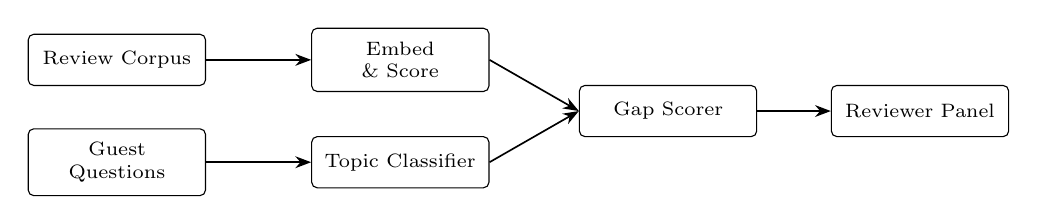
\begin{tikzpicture}[arr/.style={->, >=Stealth, semithick},
                    wbox/.style={draw, rounded corners=2pt, text centered,
                    font=\scriptsize, inner sep=5pt,
                    text width=1.9cm, minimum height=0.65cm}]

\node[wbox] (corpus)    at (0,    0.65) {Review Corpus};
\node[wbox] (signals)   at (3.6,  0.65) {Embed \& Score};
\node[wbox] (questions) at (0,   -0.65) {Guest Questions};
\node[wbox] (classify)  at (3.6, -0.65) {Topic Classifier};
\node[wbox] (scorer)    at (7.0,  0)    {Gap Scorer};
\node[wbox] (panel)     at (10.2, 0)    {Reviewer Panel};

\draw[arr] (corpus)    -- (signals);
\draw[arr] (questions) -- (classify);
\draw[arr] (signals.east)  -- (scorer.west);
\draw[arr] (classify.east) -- (scorer.west);
\draw[arr] (scorer)    -- (panel);
\end{tikzpicture}
\end{center}

\smallskip
\begin{columns}[T]
\column{0.48\textwidth}
\small\textbf{Embed \& Score:} OpenAI embeddings (coverage) + VADER (sentiment variance) +
exponential recency weighting (180-day half-life)

\column{0.48\textwidth}
\small\textbf{Gap Scorer:} Combines coverage deficit, sentiment variance, and normalised demand;
returns top-3 topics. GPT-4o-mini discovers property-specific gaps outside the fixed taxonomy.
\end{columns}

\end{frame}

% ── Slide 8: Feedback loop ───────────────────────────────────
\begin{frame}{The Feedback Loop}

\begin{columns}[T]
\column{0.46\textwidth}

\begin{center}
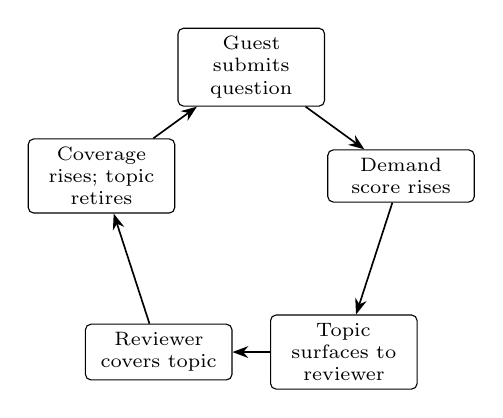
\begin{tikzpicture}[arr/.style={->, >=Stealth, semithick},
                    lbox/.style={draw, rounded corners=2pt, text centered,
                    font=\scriptsize, inner sep=3pt,
                    text width=1.65cm, minimum height=0.58cm}]
\node[lbox] (ask)     at ( 90:2cm) {Guest submits question};
\node[lbox] (demand)  at ( 18:2cm) {Demand score rises};
\node[lbox] (nudge)   at (-54:2cm) {Topic surfaces to reviewer};
\node[lbox] (covers)  at (-126:2cm){Reviewer covers topic};
\node[lbox] (retires) at (162:2cm) {Coverage rises; topic retires};
\draw[arr] (ask)     -- (demand);
\draw[arr] (demand)  -- (nudge);
\draw[arr] (nudge)   -- (covers);
\draw[arr] (covers)  -- (retires);
\draw[arr] (retires) -- (ask);
\end{tikzpicture}
\end{center}

\column{0.50\textwidth}
Retirement is \textbf{automatic}: as reviews address a topic its gap score drops
below the surfacing threshold and it stops appearing. No manual curation.

\smallskip
Each iteration raises the information floor:
\begin{itemize}
  \item Guests find answers without having to ask
  \item Reviewers contribute targeted content with the same effort
  \item Properties convert at rates that match their actual quality
\end{itemize}

\smallskip
\textbf{The supply and demand sides of information are finally connected.}

\smallskip
\textbf{Metric:} \textit{Coverage Breadth} --- fraction of topics with adequate
coverage per property, averaged across the platform.

\end{columns}

\end{frame}

% ── Slide 9: Limitations ────────────────────────────────────
\begin{frame}{Limitations and Honest Scope}

\shead{What we built and what we know still needs work}

\begin{itemize}
  \item \textbf{Topic granularity} --- the 15-category taxonomy surfaces broad nudges (e.g.\ ``Noise'').
        A reviewer writing about noise levels may still need more specific direction;
        user-submitted questions could eventually drive sub-topic resolution

  \item \textbf{Demand signal noise} --- a small number of highly engaged guests asking idiosyncratic
        questions can over-weight niche topics that are not generally relevant to most travelers

  \item \textbf{Browse-phase engagement} --- Feature 2 depends on prospective guests choosing to
        submit questions while browsing. Low engagement here weakens the demand signal and
        degrades the system to taxonomy-only nudging

  \item \textbf{Cold start} --- new properties with few reviews rely on universal taxonomy defaults;
        the system improves monotonically with review volume but starts sparse
\end{itemize}

\medskip
These are known tradeoffs, not surprises. Each has a clear improvement path
that scales with data volume and user engagement.

\end{frame}

% ── Slide 10: Summary ────────────────────────────────────────
\begin{frame}{Summary}

\begin{center}
\begin{tabular}{ll}
  \textbf{Problem}    & Reviews are the top booking signal but systematically incomplete \\[0.4em]
  \textbf{Gap}        & No system routes traveler information needs back to reviewers \\[0.4em]
  \textbf{Insight}    & Altruistic intent exists --- reviewers need direction, not pressure \\[0.4em]
  \textbf{Voice}      & Rejected: strips writing experience, turns authors into respondents \\[0.4em]
  \textbf{Feature 1}  & Real-time gap checklist with crossoff (supply side) \\[0.4em]
  \textbf{Feature 2}  & Guest question submission, demand-weighted (demand side) \\[0.4em]
  \textbf{Loop}       & Coverage rises as gaps are filled; topics retire automatically \\[0.4em]
  \textbf{Stack}      & Embeddings $\cdot$ VADER $\cdot$ GPT-4o-mini $\cdot$ Streamlit \\[0.4em]
  \textbf{Limits}     & Broad categories, demand noise, browse engagement, cold start \\[0.4em]
  \textbf{Metric}     & Coverage Breadth: fraction of topics with adequate coverage per property \\
\end{tabular}
\end{center}

\bigskip
\begin{center}
  \large\textbf{Ask What Matters}\\[0.3em]
  \normalsize Reviews are only as useful as the questions they answer.
\end{center}

\end{frame}

\end{document}
